% Benvenuti nel template per le relazioni di Sperimentazioni di Fisica 1 del corso triennale in Astronomia dell'Università di Padova.
% Per compilarlo, cliccate su Menu, selezionate come compilatore "pdfLaTeX", TeX Live Version 2020 (o uno degli altri, whatever works), e come documento principale "Relazione.tex"

%%% Preambolo del documento %%%
% Non toccate questa roba, a meno che non siate abbastanza sgamati da sapere quello che state facendo, tipo vi piacciono di più certi pacchetti rispetto ad altri, o magari ve ne manca qualcuno.
\documentclass[a4paper, titlepage]{article}
\usepackage[T1]{fontenc}
\usepackage[utf8]{inputenc}
\usepackage[italian]{babel}
\usepackage{amsmath}
\usepackage{listings}
\usepackage{textcomp}
\usepackage{multirow}
\usepackage{multicol}
\usepackage{booktabs}
\usepackage{graphicx}
\usepackage{floatflt}
\usepackage{epsfig}
\usepackage{pstricks}
\usepackage{subfigure}
\usepackage[labelfont=bf, font=scriptsize]{caption}
\usepackage[italian]{varioref}
\usepackage[suftesi]{frontespizio}
\usepackage{color}
\usepackage{tikz}
\usepackage{caption}
\usepackage{pgfplots}
\usepackage{comment}
\usepackage{lipsum}
\pgfplotsset{compat=1.16}

%%% Il documento vero e proprio %%%
\begin{document}

%%% Frontespizio %%%
% Questa serie di comandi genera il frontespizio della relazione.
% Cambiate: l'Anno Accademico, Data e Titolo della relazione, il nome degli appartenenti al gruppo con annessa matricola e mail istituzionale. Se siete due o quattro in gruppo, basta togliere/inserire una riga Candidato.
% NON toccate i comandi con accanto con CTT (Can't Touch This).
% !!! NOTA PER LA CORRETTA VISUALIZZAZIONE DEL FRONTESPIZIO. !!!
% Quando si compila un file su Overleaf, per velocizzare le successive compilazioni questi genera una cache, e da questa prende gli elementi che, a senso suo, non sono cambiati nel testo. Quindi per quanto vi possiate ostinare a compilare, vedrete sempre il primo frontespizio che ha compilato (quello con NomeCognome etc etc) e non le ultime modifica.
% Come evitare ciò, e visualizzare il frontespizio con i vostri nomi, cognomi e numeri matricola? Così: cliccate sull'icona accanto a Recompile, quella con il simbolo del documento, e successivamente sul simbolo del cestino (Clear cached files). Liberate la cache, modificate il frontespizio, e ricompilate. Così dovreste riuscire a vedere nel file compilato le vostre modifiche al frontespizio. Ricordatevi di svuotare la cache del file Overleaf ogni volta che volete modificare qualcosa nel frontespizio.
\begin{frontespizio}
\Universita{Padova} % CTT
\Logo{Figure/logo_polimi} % CTT
\Divisione{Statistica} % CTT
\Corso[Laurea]{Ingegneria Fisica} % CTT, a meno che non cambi la denominazione del corso
\Annoaccademico{2020-2021}
\Titoletto{Progetto d'esame} % CTT
\Titolo{Analisi statistica degli esopianeti}
\Sottotitolo{Un'analisi statistica sui parametri determinanti l'abitabilità di pianeti extra solari}
\NCandidati{Gruppo di lavoro} % CTT
\Candidato[959859]{Rolleri Gabriele, \textsf {gabriele.rolleri@mail.polimi.it}}
\Candidato[954997]{Sergenti Filippo, \textsf {filippo.sergenti@mail.polimi.it}}
\Candidato[960718]{Zhang Giovanni, \textsf {giovanni.zhang@mail.polimi.it}}
\NRelatore{Docente}{} % CTT
\Relatore{Prof. Alessandro Toigo} % CTT, a meno che non sia cambiato il Prof.
\end{frontespizio}
\IfFileExists{\jobname-frn.pdf}{}{%
\immediate\write18{pdflatex \jobname-frn}} % ASSOLUTAMENTE CTT, è il comando che materialmente vi genera il frontespizio.

%%% Indice %%%
\tableofcontents

\newpage
%%% Sezioni %%%
% Qui inizia la relazione vera e propria.
% Le Sezioni sono singoli file .tex dentro la cartella Sezioni. Potete a libera scelta scrivere tutto su un singolo file e chiamare all'interno di questi con il comando \section{} le varie sezioni, oppure dividere le singole sezioni in più file Sezione_i.tex, e poi inserirle tutte con \input{Sezioni/Sezione_i.tex} per i = 1 ... N
\section{Introduzione}
Questa è l'introduzione


	
\section{Statistica descrittiva}
I sistemi planetari più comunemente rilevati sono decisamente quelli a una stella a un pianeta, I sistemi planetari più comunemente rilevati sono decisamente quelli a una stella a un pianeta, I sistemi planetari più comunemente rilevati sono decisamente quelli a una stella a un pianeta, I sistemi planetari più comunemente rilevati sono decisamente quelli a una stella a un pianeta, 
\begin{wrapfigure}{l}{0.35\textwidth}

   
	\centering
    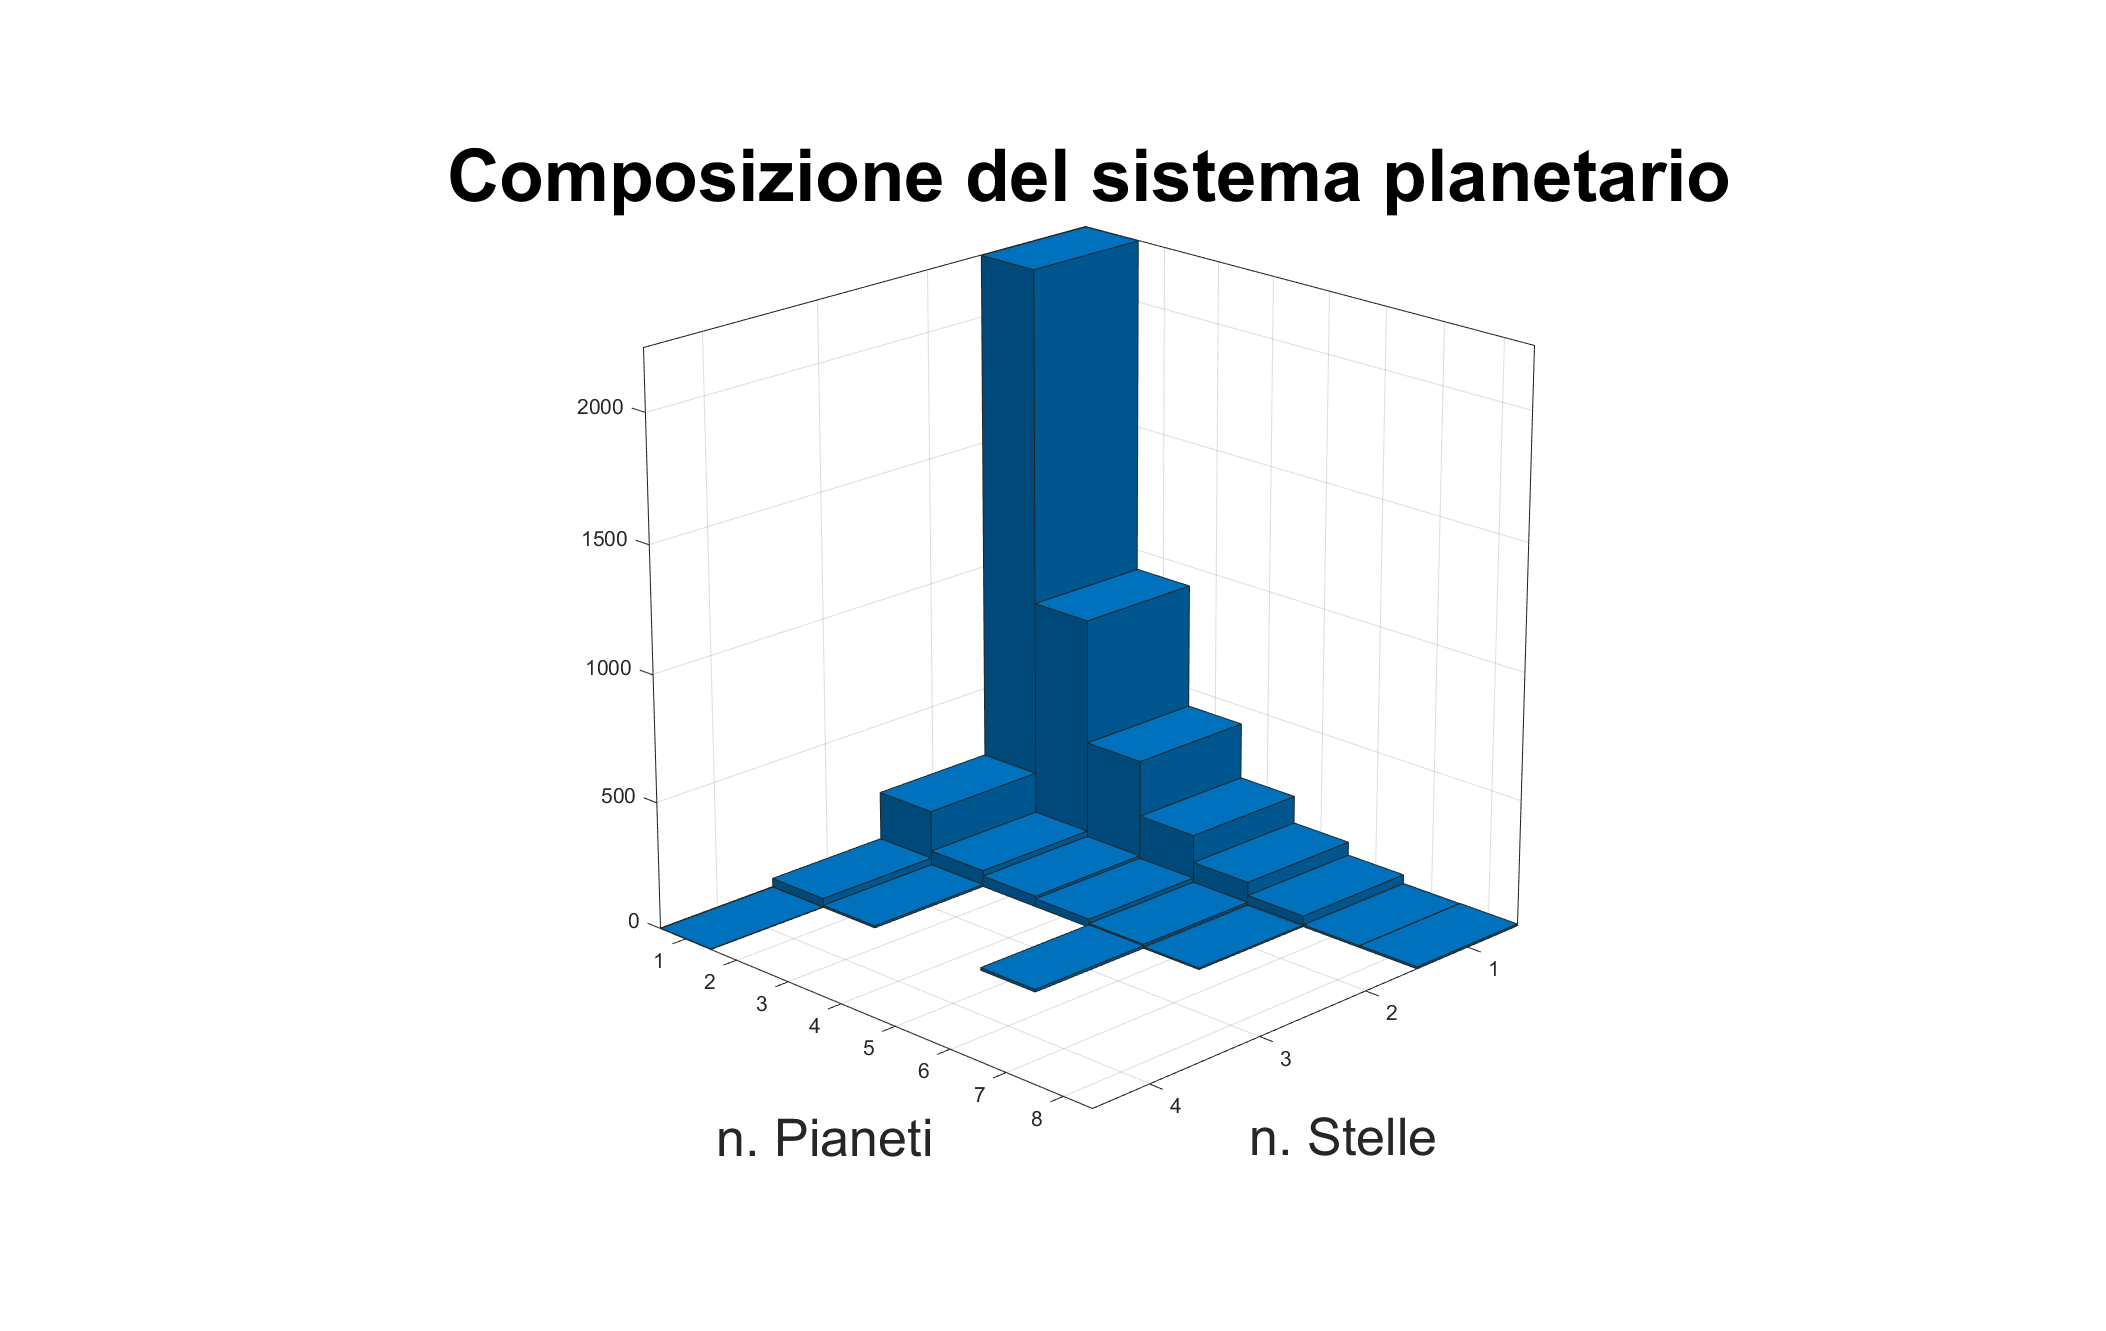
\includegraphics[width=0.35\textwidth]{Figure/hist_sistema_planetario} 
	
   

\end{wrapfigure}
I sistemi planetari più comunemente rilevati sono decisamente quelli a una stella a un pianeta, I sistemi planetari più comunemente rilevati sono decisamente quelli a una stella a un pianeta, I sistemi planetari più comunemente rilevati sono decisamente quelli a una stella a un pianeta, I sistemi planetari più comunemente rilevati sono decisamente quelli a una stella a un pianeta, I sistemi planetari più comunemente rilevati sono decisamente quelli a una stella a un pianeta, I sistemi planetari più comunemente rilevati sono decisamente quelli a una stella a un pianeta, I sistemi planetari più comunemente rilevati sono decisamente quelli a una stella a un pianeta, 
\section{Test d'ipotesi}
Qua faremo un test d'ipotesi
\section{Regressione}
La regressione va qua

\newpage
%%% Appendici %%%
% Eventuali appendici vanno qui. Se non avete appendici da inserire, togliete/commentate queste righe.
%\appendix
%\input{Sezioni/Appendice.tex}	
\bibliography{progetto}
\end{document}

% Credits: basato sulle relazioni di laboratorio di Nicola Bellucco, Marco Codato e Erica Korb.